\documentclass[a4paper, 12pt]{article}
\usepackage{graphicx} % Required for inserting images
\usepackage{textcomp}
\usepackage{fullpage}
\usepackage{amsmath}
\usepackage{xcolor}
\usepackage{float}
\usepackage{geometry}
\usepackage{biblatex}
\geometry{margin=1in}
\usepackage{enumitem}
\usepackage{hyperref}
\usepackage{microtype}
\usepackage{gensymb}
\usepackage{parskip}
\usepackage{tikz}
\usepackage{caption}
\usepackage{cancel}
\usepackage{nicefrac}
\hypersetup{
    colorlinks=true,        % Enable colored links
    linkcolor=teal,         % Set color for internal links
    citecolor=teal,         % Set color for citations
    filecolor=teal,         % Set color for file links
    urlcolor=teal           % Set color for URLs
}

\usepackage[version=4]{mhchem}

\title{Fundamentals}
\author{BIOS 1006}
\date{17 June 2025}

\begin{document}

\maketitle

\section*{Objectives}

\begin{itemize}
\item Know all definitions.
\item Know the basic atoms that comprise biological systems. (CHNOPS)
\item Describe why carbon is ideal for forming the skeleton of biomolecules.
\item Name and draw the common functional groups found in biomolecules.
\item Recognize different molecular representations and draw abbreviated and expanded structural formulae.
\item Describe the four basic building that comprise biological systems, their different sub-classifications, and the four major classes of biomolecules that they form. Identify to which class of the four basic building blocks a small molecule belongs or is related.
\item Describe the properties of water that make it an ideal solute for life.
\item Describe the properties of hydrogen bonds and what is required for them to be formed.
\item Describe the three types of “weak” interactions, the types of groups that participate in these interactions and the role they play in solvation and biomolecular structure.
\item Describe Lennard-Jones plots and use them to describe and predict interactions between molecules.
\item Describe the hydrophobic effect and van der Waals interactions and describe their different roles in biomolecular structure.
\item Describe the properties and principles of buffers and buffering capacity.
\item Calculate the pH from the concentration of \ce{H+} and vice versa.
\item Calculate the pH, pKa or the amounts of acid and conjugate base using the Henderson-Hasselbalch equation.
\item Predict protonation state of a group based on it pKa and the buffer pH.
\item Describe the physiologically important buffers.
\end{itemize}

\newpage

\section*{Definitions}

\begin{description}
\item [electrostatic] involves charges
\item [functional groups] specific groups of atoms within molecules that are responsible for the molecule's characteristic chemical reactions
\item [solute] in a solution, dissolved in a solvent
\item [solvent] in a solution, dissolves the solute
\item [weak interactions] weaker, transient interactions that are additive and can become stronger
\end{description}

\newpage

\section*{The biological building blocks}

\begin{figure}[H]
\centering
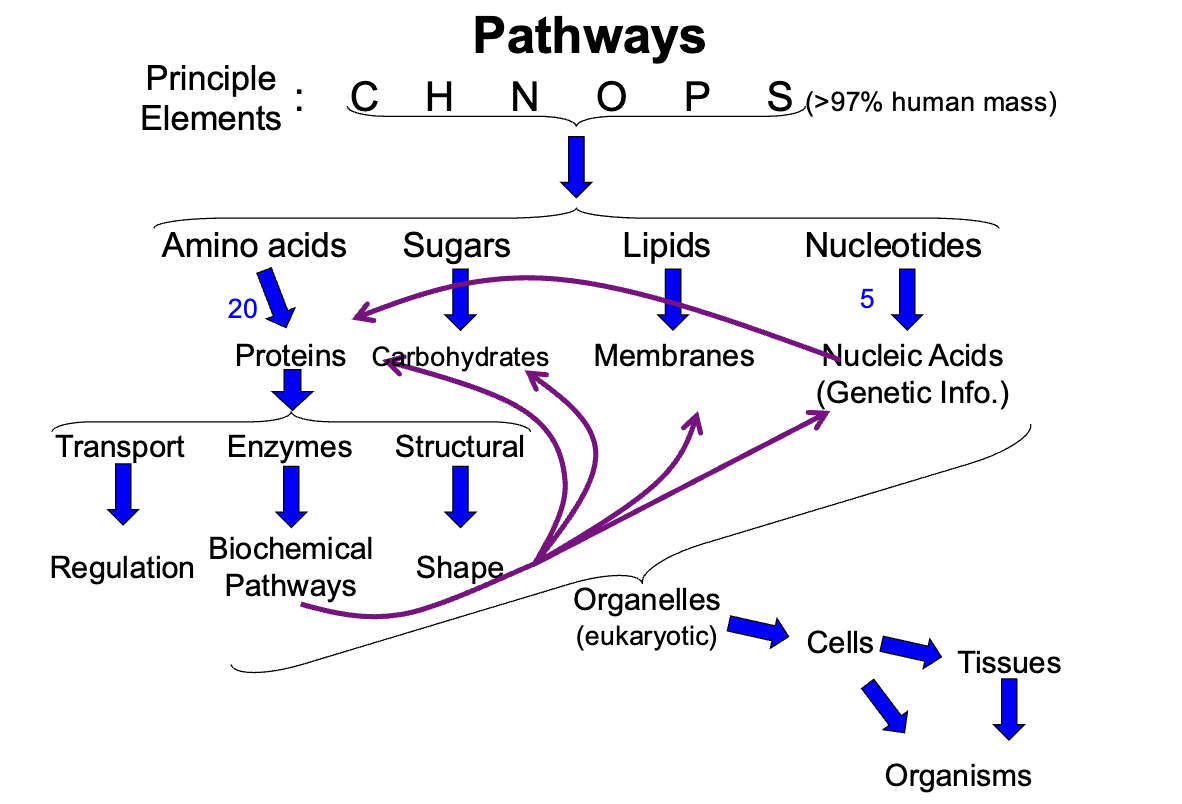
\includegraphics[width=0.8\textwidth]{pathways}
\end{figure}

\subsection*{Functional groups}

(R denotes a generic hydrocarbon chain)

Memorize!

\begin{figure}[H]
\centering
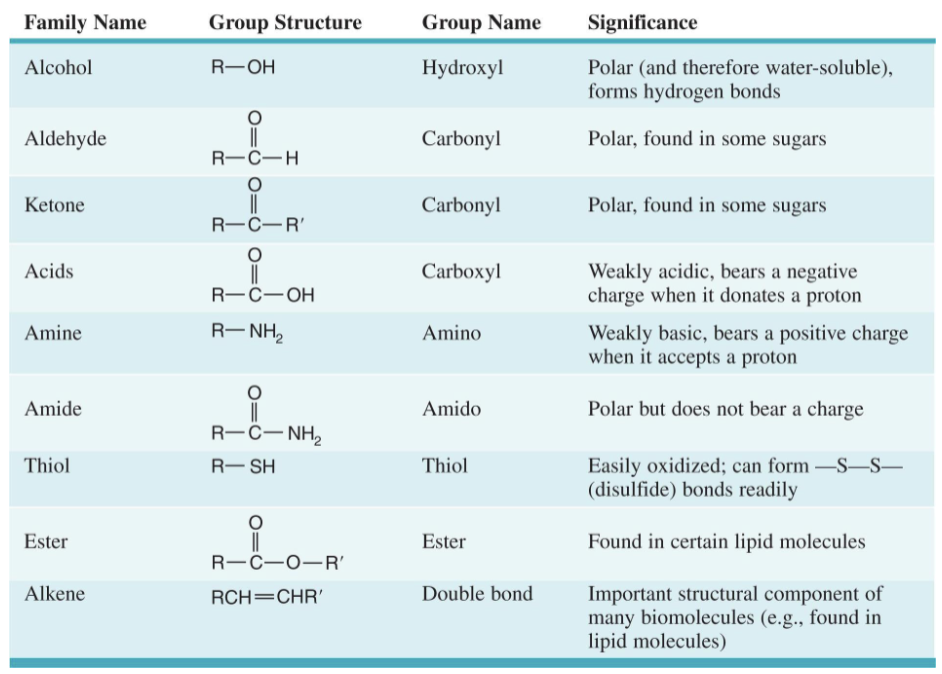
\includegraphics[width=0.8\textwidth]{functionalgroups}
\end{figure}

+ \textbf{phosphate} (\ce{PO4^3-})

\begin{itemize}
\item \textbf{Hydroxyl} + \textbf{carbonyl} $\to$ \textbf{carboxyl}
\item \textbf{Amine} + \textbf{carbonyl} $\to$ \textbf{amide}
\item \textbf{Aldehyde} has carboxyl at the \textbf{end}; \textbf{ketone} has it in the \textbf{middle}
\end{itemize}

\subsection*{Representations of molecules}

\begin{figure}[H]
\centering
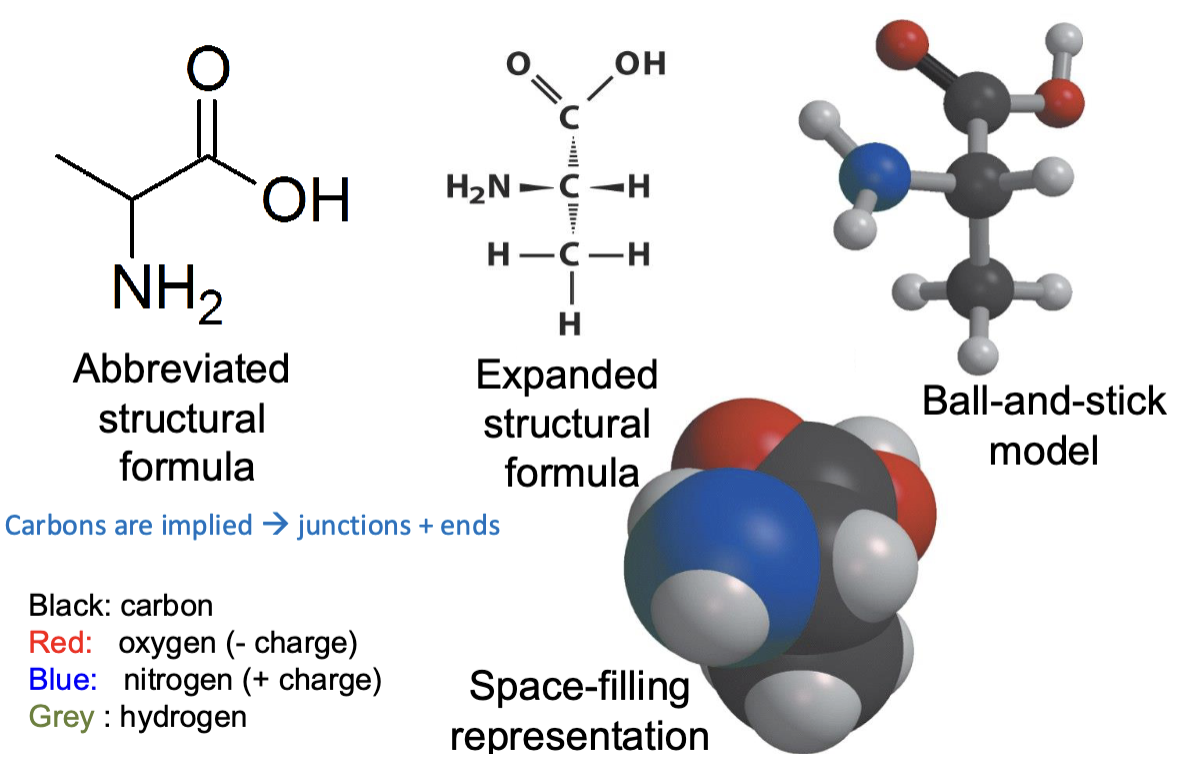
\includegraphics[width=0.8\textwidth]{models}
\end{figure}

\subsection*{The four major classes}

\subsubsection*{Amino acids}

\begin{itemize}
\item Hundreds of naturally occurring forms
\item Defined by the presence of amine and carboxylic acid groups
\item Classified based on the proximity of these groups
\item Three different classes: $\alpha$, $\beta$, and $\gamma$ based on which carbon is attached to the amine (closest to the central carbon is $\alpha$, next is $\gamma$, etc.)
\item $\alpha$ amino acid (most common): \textbf{amine} attached to \textbf{$\alpha$ carbon} (1 away from the central carbon), carboxyl and an \textbf{R group} (side chain, 20 different common types)
\item \textbf{Peptide} or \textbf{amide} bonds link amino acids together (form amide group with the carboxyl group + amine group)
\end{itemize}

\subsubsection*{Sugars (carbohydrates)}

\begin{itemize}
\item Molecules containing carbonyl and hydroxyl functional groups
\item Two classes: \textbf{ketose} and \textbf{aldose} sugars (carbonyl in the middle = ketose, at the end = aldose, same as functional groups)
\item Hydrated carbons
\item Very hydrophilic
\end{itemize}

\subsubsection*{Lipids}

\begin{itemize}
\item Soluble in hydrophobic solutions
\item Do not polymerize but form higher order structures
\item Fatty acids
\end{itemize}

\subsubsection*{Nucleotides}

\begin{itemize}
\item 3 basic components: phosphate group(s), ribose, nitrogenous base
\item Polymerize into: DNA (deoxyribose, adenosine, cytosine, guanine, thymine); RNA (ribose, adenosine, cytosine, guanine, uracil)
\item \textbf{Purines} (2 rings) and \textbf{pyrimidines} (1 ring)
\item Mnemonics: ``Pure As Gold'' (adenine and guanine are purines) and ``CUT the Py'' (cytosine, thymine, and uracil are pyrimidines)
\end{itemize}

\newpage

\section*{Water (\ce{H2O}): the biological solvent}

\subsection*{Physical properties of water}

\begin{itemize}
\item Solvent characteristics
\item Non-compressible
\item Chemical stability
\item Biochemical reactant
\item Hydration of molecules
\item Participates in biomolecular interactions
\item Ice floats
\item High boiling and freezing temperatures
\item High heat of vaporization
\item High specific heat capacity
\item High surface tension
\item Dissolves molecules with ionizable or polarizable functional groups but cannot dissolve nonpolar or hydrophobic molecules
\end{itemize}

\subsection*{Molecular properties of water}

\begin{itemize}
\item \textbf{Tetrahedral} electron geometry (104.5 degrees),  sp$^3$ hybridized, 0.99 Å from H to O
\item Electronegativity results in the formation of \textbf{polar bonds}
\item Forms \textbf{hydrogen bonds} (hydrogen is attracted to the lone pair electrons of an oxygen from another molecule)
\end{itemize}

\subsection*{Properties of hydrogen bonds}

\begin{itemize}
\item Hydrogen bonds in between casual interaction and covalent interaction in terms of proximity
\item Both covalent and electrostatic properties
\item Collinear orientation (present in a straight line)
\item Other orientations possible but not as strong
\item Electrostatic interaction
\item Atoms involved share electrons
\item In liquid water, 3.4 neighbors on average (4 in ice)
\end{itemize}

\subsection*{Weak interactions}

\begin{itemize}
\item Weak interactions are constantly being formed and broken between biomolecules (more transient)
\item Additive (can become strong)
\item Essential for rapid communication
\item Allows for flexibility
\item Three types of weak electrostatic interactions
\begin{itemize}
\item \textbf{Salt bridges} (ionic)
\item \textbf{Van der Waals interactions}
\item \textbf{Hydrogen bonds}
\end{itemize}
\end{itemize}

\subsection*{Relative strengths of interactions}
Strongest to weakest
\begin{itemize}
\item Int\textbf{ra}molecular forces
\begin{itemize}
\item Ionic bonds
\item Covalent bonds
\end{itemize}
\item Int\textbf{er}molecular forces (IMFs)
\begin{itemize}
\item Ionic interactions and salt bridges
\item Van der Waals forces
\item Hydrogen bonds
\item Dipole-dipole interactions
\item London dispersion forces (LDFs)
\end{itemize}
\end{itemize}

\subsubsection*{Salt bridges and ionic interactions}

\begin{itemize}
\item One positive interacting with one negative with full electrical charges (ionic bonds are NOT salt bridges)
\item Interaction strength calculated from Coulomb's law: $$ F = \frac{1}{4 \pi \varepsilon_0 } \frac{q_1q_2}{\varepsilon_r r^2}$$
\begin{itemize}
\item $F$ is interaction strength
\item $q_1$ and $q_2$ are signed charges
\item $r$ is the distance between centers
\item $\varepsilon_r$ is the dielectric constant
\item All others are constants
\end{itemize}
\item Water is good at breaking ionic bonds
\item \textbf{Hydration shells} prevent ionic bonds from reforming
\end{itemize}

\end{document}